% Source: Code/yolo-ablation-bench/precision_report.tex

\documentclass[border=4pt]{standalone}
\usepackage{amssymb}
\usepackage[T1]{fontenc}
\usepackage{graphicx}
\usepackage{helvet}
\usepackage{lmodern}
\usepackage{pgfplots}
\usepackage{pgfplotstable}
\usepackage{tikz}
\usepackage[dvipsnames,table]{xcolor}
\pgfplotsset{compat=1.18}

\definecolor{garnet}{HTML}{73000A}
\definecolor{midgray}{gray}{0.35}
\definecolor{lightgray}{gray}{0.8}
\definecolor{dlacolor}{HTML}{2E7D32}
\definecolor{gpucolor}{HTML}{1565C0}
\definecolor{fp32color}{HTML}{9E9E9E}
\definecolor{fp16color}{HTML}{FF9800}
\definecolor{int8color}{HTML}{4CAF50}


\newcommand{\headline}[1]{\textcolor{garnet}{\Large\bfseries #1}}
\newcommand{\subhead}[1]{\textcolor{midgray}{\large #1}}
\newcommand{\fpthirtytwo}[1]{\textcolor{fp32color}{\textbf{#1}}}
\newcommand{\fpsixteen}[1]{\textcolor{fp16color}{\textbf{#1}}}
\newcommand{\inteight}[1]{\textcolor{int8color}{\textbf{#1}}}
\newcommand{\gpu}[1]{\textcolor{gpucolor}{\textbf{#1}}}
\newcommand{\dla}[1]{\textcolor{dlacolor}{\textbf{#1}}}

\begin{document}
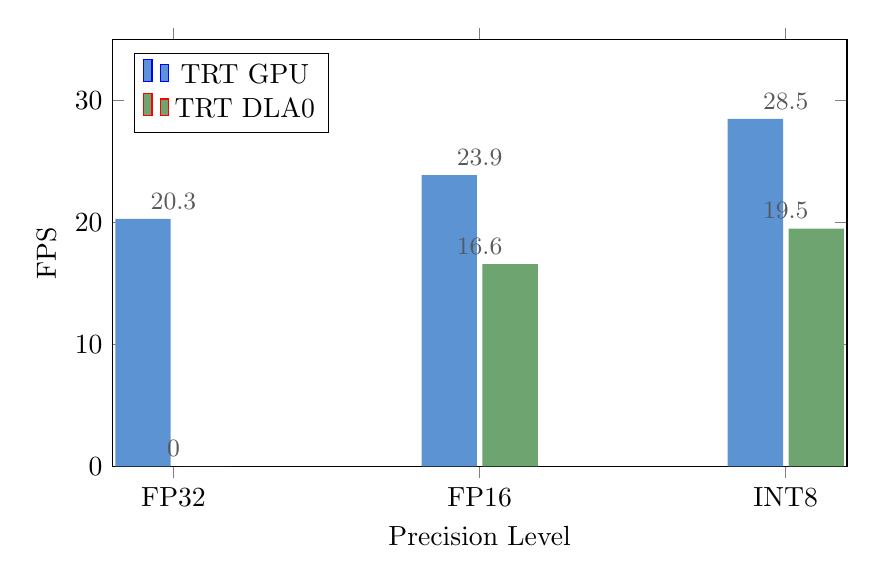
\begin{tikzpicture}
  \begin{axis}[
    width=0.9\textwidth,
    height=7cm,
    ybar,
    bar width=20pt,
    xlabel={Precision Level},
    ylabel={FPS},
    symbolic x coords={FP32,FP16,INT8},
    xtick=data,
    legend pos=north west,
    ymin=0, ymax=35,
    nodes near coords,
    every node near coord/.style={font=\small, color=midgray, anchor=south},
  ]
    % GPU
    \addplot+[fill=gpucolor!70, draw=none] coordinates {
      (FP32, 20.3) (FP16, 23.9) (INT8, 28.5)
    };
    \addlegendentry{TRT GPU}
    % DLA
    \addplot+[fill=dlacolor!70, draw=none] coordinates {
      (FP32, 0) (FP16, 16.6) (INT8, 19.5)
    };
    \addlegendentry{TRT DLA0}
  \end{axis}
\end{tikzpicture}
\end{document}
